\section{Evaluation}

\subsection{Procedure}

We conducted a qualitative usability study to understand how \Glspl{name}-generated \glspl{exp} affected programmers' ability to perform code modification tasks with online example code.
We recruited 9 programmers from university listservs for undergraduate and graduate students in computer science and information science.
All participants had at least two years of programming experience, with a median of 4 years of experience in their longest-used language.  Participants were asked to explain their actions via think-aloud method which was audio-recorded, and their actions were screen-captured and analyzed post-hoc. 

Each participant attempted 8 code modification tasks (plus 2 practice tasks) using two different languages: CSS selectors and \texttt{wget}.
For each language the 4 coding tasks increased in difficulty with the fourth being especially tricky.
We created snippets consisting of a block of code and optionally  explanatory text and comments for each task, based on  existing online programming help.

Each code modification task consisted of the following steps:
\begin{enumerate}
\item Read a task --- e.g., \emph{write a CSS selector that selects only elements of class \texttt{myInput}.}
\item View a snippet with some clue about the task.
E.g., in Figure~\ref{fig:study_snippet}, the participant was shown a snippet containing CSS selectors that choose elements of class \emph{myCheckbox} without explaining the syntax.
\item Write and test the code in a sandbox we provided.
\end{enumerate}
After reading the snippet, to solve the task, participants could use any resources they wanted to, including searching the web.
Participants were told they would have 5 minutes for each task; when participants had extra time, if  they had not completed the task, we often asked them to continue so we could observe their problem-solving process. When in the micro-explanation condition participants were asked to find and view all \glspl{exp} for the source code after reading the snippet.

\begin{figure}
\centering
\framebox{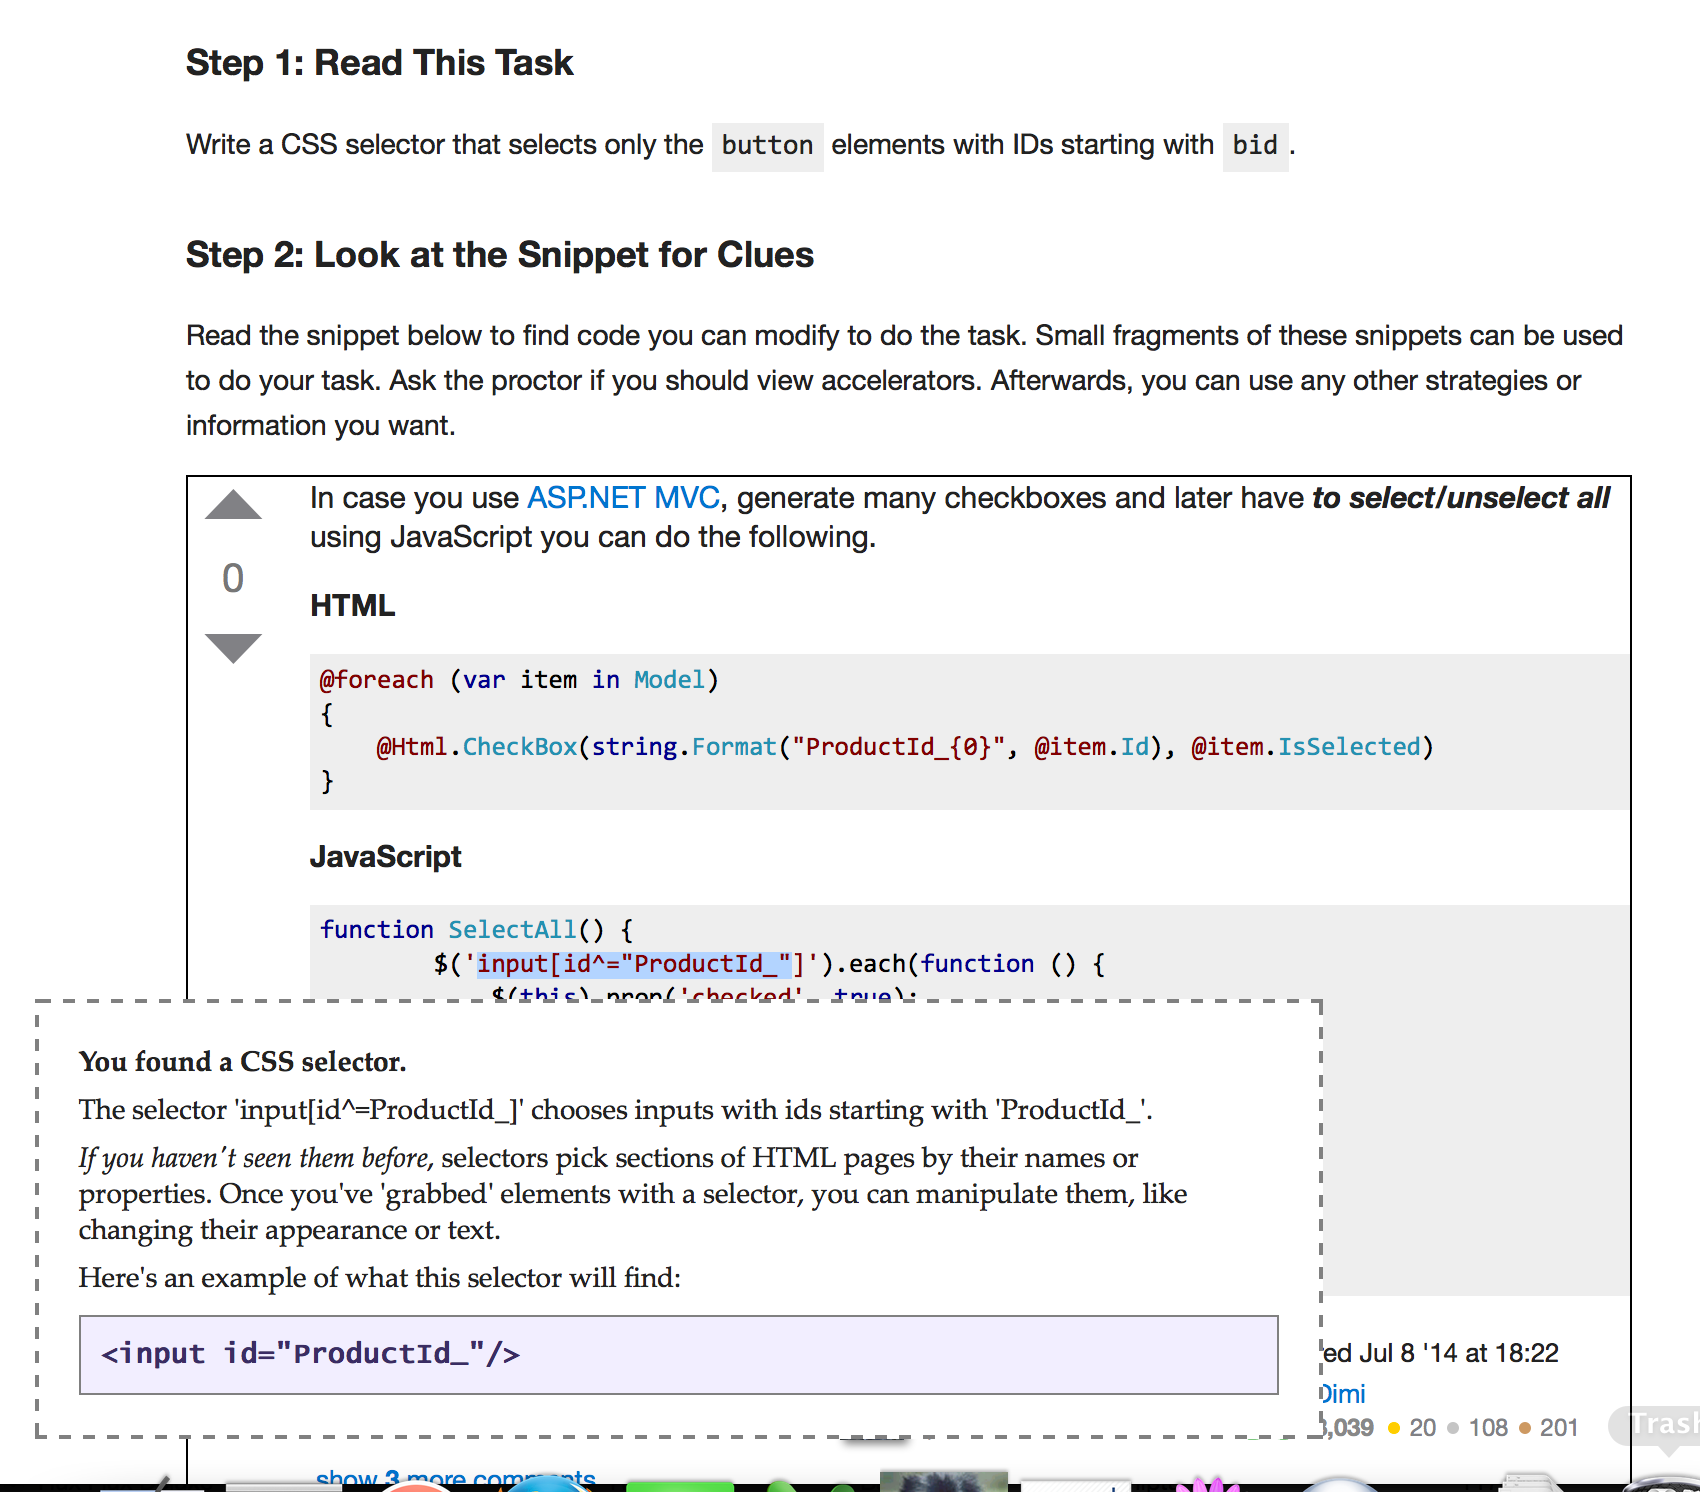
\includegraphics[width=\columnwidth]{figures/study_snippet}}
\caption{An example snippet shown as a clue for a code modification task, accompanied by a micro-explanation that a participant in our study would have viewed if they were instructed to do so in this task.}
\label{fig:study_snippet}
\end{figure}

Participants viewed \glspl{exp} for alternating tasks so we could observe differences in how they approached the tasks with and without micro-explanations; exposure to micro-explanations was counter-balanced across participants. 

%%This ordering was counterbalanced across participants so that we could see all tasks performed both with and without \gls{name}-generated \glspl{exp}.



\subsection{Results}

Our primary goal in observing participants was to determine if \gls{name}-generated \glspl{exp} were helpful  during code modification tasks and reduced the need to reference additional documentation.
In the discussion below, we refer to individual participants as $P{1-9}$.

\subsubsection{ \Glspl{exp} Help Programmers Modify Code Without Using Other Documentation}

\begin{figure}
\centering
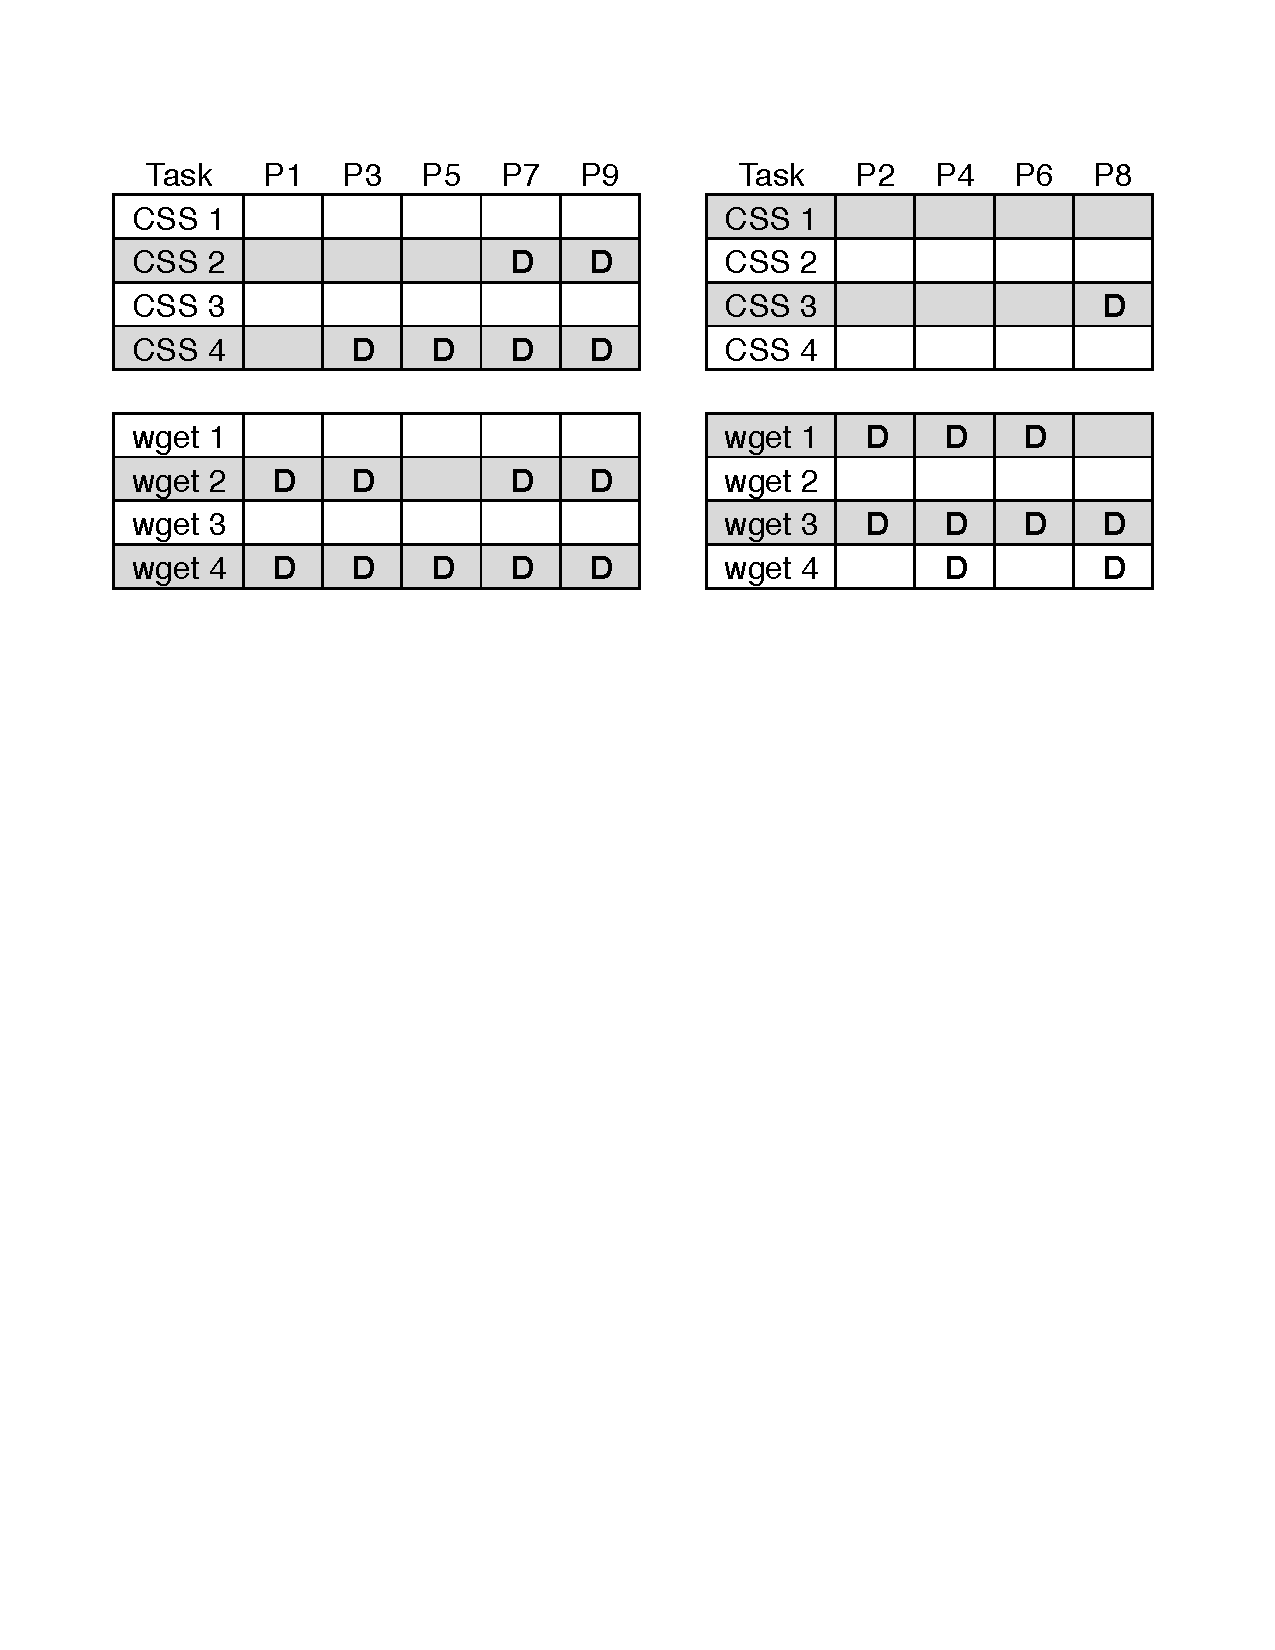
\includegraphics[width=\columnwidth]{figures/doc_accesses}
\caption{
Tasks for which participants sought additional documentation beyond the snippet. In white rows, participants used \glspl{exp}; in gray rows, they did not.
A cell is marked with the letter `D' if a participant accessed external documentation during that task.
}
\label{fig:doc_accesses}
\end{figure}

When using the micro-explanations, 34 out of 36 tasks, or 94\% did not require external documentation.  However, for those tasks where micro-explanations were not available, 63\% of the time participants did indeed access external resources in order to complete the task.  The wget tasks especially required external help, with man pages and other resources being accessed in 89\% of cases.  
A detailed breakdown of external document usage is shown in Figure \ref{fig:doc_accesses}. 


%%In total, out of 72  tasks, participants sought out additional documentation a total of 25 times (Figure~\ref{fig:doc_accesses}).
%%In all wget tasks and in the fourth CSS selector task, a majority of participants without \glspl{name} viewed documentation at some point while trying to find a solution to the problem.
%%In the all 4 CSS selector tasks and the first 3 wget tasks, no participants with access to the \glspl{exp} sought additional documentation in order to solve the problem.

%Only in the final wget task did any participants with access to \glspl{name} seek documentation.


These preliminary results suggest that the micro-explanations are effective at reducing the need to switch contexts to find relevant programming help  for completing some programming tasks. 
The \gls{exp} aided the programmers in several ways:

{\bf Reducing need to access external documentation.}
Participants were  able to identify which flags had to be removed from wget commands without consulting external documentation, despite not having used the wget before ($P4$).
For others, the \gls{exp} affirmed a guess that the participant already had about how to construct a CSS selector ($P1$).

{\bf Context-relevant pattern matching.}
One participant noted that the \glspl{exp} helped  to map flags for the wget command line to the higher-level intent of the task ($P4$). 
For the most complex CSS selector task (see Figure \ref{fig:study_snippet}), two participants noted
that the example HTML shown in the \gls{exp} 
provided a pattern of what fields needed to be changed  from the selector in the snippet to capture the element and ID required by the task prompt ($P2$, $P4$).

{\bf Learning programming concepts.}
For another participant with little previous experience with CSS selectors, a \gls{exp} in  the first task provided him with the knowledge needed to write the selector for the next two tasks, one task for which he was not allowed to view \glspl{exp} ($P5$).

\subsubsection{Programmers Without \Gls{exp} Searched External Documentation}

Some of the difficulties participants faced in the no-\gls{exp} condition  highlight the benefits of in-situ help.
Some participants had difficulty searching for programming help on a web search engine (Google) and using the seach results.
One participant could not express the symbols `\texttt{\^{}=}' as a query term when searching for what  this pattern signifies in CSS selectors.
Her follow-up queries with English language query terms  yielded search results that were not relevant ($P3$).

Participants also had difficulty navigating conventional forms of programming help.
When looking for the \texttt{-r} flag in the man page for wget ($P2$, $P4$), participants found that a page-internal  search for the flag yielded so many matches that it was difficult to find the desired definition.
The description of the \texttt{-N} timestamp flag that was relevant to the code modification task was not directly adjacent to where the flag was introduced, causing one participant to overlook this information, even though it was only 10 lines away ($P3$).

These results underscore the usefulness of context-relevant explanations located within the tutorial text itself.

\subsubsection{Opportunities for Improvement}
In those cases where the \gls{exp} did not aid programmers, there were a few primary causes.

{\bf No visual affordances.} We did not place  visible cues showing where explanations were available.
Programmers may fail to find micro-explanations since they have to be explicitly invoked through a right-click.
Although $P2$ eventually found a micro-explanation that led him to writing a successful CSS selector for the most difficult CSS task, he had to click around the snippet to find it, and did so only upon being reminded by the experimenter that he had not viewed all the \glspl{exp} in the snippet ($P2$).  We plan to experiment with providing visual affordances for the presence of \glspl{exp} in future.


{\bf Selection region ambiguity.}
The leniency of our algorithm for matching a text selection to an explained code fragment caused confusion for programmers about which fragments would be explained on each page ($P1$, $P2$, $P5$).
For the same reason, explanations generated did not always match the fragment selected ($P1$, $P3$, $P5$).
For example, one participant selected the text \texttt{<p>} for which no explanation was generated by the explanation server, because no CSS selector starts with a less-than sign.
However, our selection matching algorithm matched this string to the \texttt{p.mainPageMeters} selector for which an explanation \emph{had} been generated by the server.  As a result, this participant viewed an irrelevant explanation for the code fragment he was viewing ($P5$).  More work is required to determine the right balance of fuzziness for the matching algorithm, with perhaps a drop-down menu of choices for alternative matches.

{\bf Incomplete explanations.} The  \gls{exp} text may not include enough detail to help programmers  develop adequate mental models of unfamiliar material. For instance,
even after completing all 4 CSS selector tasks, $P5$ appeared to believe that CSS selectors were HTML elements themselves, rather than labels that could fetch them, perhaps confused by the example HTML produced in each \gls{exp} ($P5$).  That said, the idea of \gls{exp} can be expanded by adding links to fuller tutorial material.